
\documentclass[a4paper,11pt]{article}
\usepackage[a4paper, margin=8em]{geometry}

% usa i pacchetti per la scrittura in italiano
\usepackage[french,italian]{babel}
\usepackage[T1]{fontenc}
\usepackage[utf8]{inputenc}
\frenchspacing 

% usa i pacchetti per la formattazione matematica
\usepackage{amsmath, amssymb, amsthm, amsfonts}

% usa altri pacchetti
\usepackage{gensymb}
\usepackage{hyperref}
\usepackage{standalone}

\usepackage{colortbl}

\usepackage{xstring}
\usepackage{karnaugh-map}

% imposta il titolo
\title{Computer Architectures notes}
\author{Luca Seggiani}
\date{2026}

% imposta lo stile
% usa helvetica
\usepackage[scaled]{helvet}
% usa palatino
\usepackage{palatino}
% usa un font monospazio guardabile
\usepackage{lmodern}

\renewcommand{\rmdefault}{ppl}
\renewcommand{\sfdefault}{phv}
\renewcommand{\ttdefault}{lmtt}

% circuiti
\usepackage{circuitikz}
\usetikzlibrary{babel}

% testo cerchiato
\newcommand*\circled[1]{\tikz[baseline=(char.base)]{
            \node[shape=circle,draw,inner sep=2pt] (char) {#1};}}

% disponi il titolo
\makeatletter
\renewcommand{\maketitle} {
	\begin{center} 
		\begin{minipage}[t]{.8\textwidth}
			\textsf{\huge\bfseries \@title} 
		\end{minipage}%
		\begin{minipage}[t]{.2\textwidth}
			\raggedleft \vspace{-1.65em}
			\textsf{\small \@author} \vfill
			\textsf{\small \@date}
		\end{minipage}
		\par
	\end{center}

	\thispagestyle{empty}
	\pagestyle{fancy}
}
\makeatother

% disponi teoremi
\usepackage{tcolorbox}
\newtcolorbox[auto counter, number within=section]{theorem}[2][]{%
	colback=blue!10, 
	colframe=blue!40!black, 
	sharp corners=northwest,
	fonttitle=\sffamily\bfseries, 
	title=Theorem~\thetcbcounter: #2, 
	#1
}

% disponi definizioni
\newtcolorbox[auto counter, number within=section]{definition}[2][]{%
	colback=red!10,
	colframe=red!40!black,
	sharp corners=northwest,
	fonttitle=\sffamily\bfseries,
	title=Definition~\thetcbcounter: #2,
	#1
}

% disponi codice
\usepackage{listings}
\usepackage[table]{xcolor}

\definecolor{codegreen}{rgb}{0,0.6,0}
\definecolor{codegray}{rgb}{0.5,0.5,0.5}
\definecolor{codepurple}{rgb}{0.58,0,0.82}
\definecolor{backcolour}{rgb}{0.95,0.95,0.92}

\lstdefinestyle{codestyle}{
		backgroundcolor=\color{black!5}, 
		commentstyle=\color{codegreen},
		keywordstyle=\bfseries\color{magenta},
		numberstyle=\sffamily\tiny\color{black!60},
		stringstyle=\color{green!50!black},
		basicstyle=\ttfamily\footnotesize,
		breakatwhitespace=false,         
		breaklines=true,                 
		captionpos=b,                    
		keepspaces=true,                 
		numbers=left,                    
		numbersep=5pt,                  
		showspaces=false,                
		showstringspaces=false,
		showtabs=false,                  
		tabsize=2
}

\lstdefinestyle{shellstyle}{
		backgroundcolor=\color{black!5}, 
		basicstyle=\ttfamily\footnotesize\color{black}, 
		commentstyle=\color{black}, 
		keywordstyle=\color{black},
		numberstyle=\color{black!5},
		stringstyle=\color{black}, 
		showspaces=false,
		showstringspaces=false, 
		showtabs=false, 
		tabsize=2, 
		numbers=none, 
		breaklines=true
}

\lstdefinelanguage{x86}{ 
  keywords={AAA, AAD, AAM, AAS, ADC, ADCB, ADCW, ADCL, ADD, ADDB, ADDW, ADDL, AND, ANDB, ANDW, ANDL,
        ARPL, BOUND, BSF, BSFL, BSFW, BSR, BSRL, BSRW, BSWAP, BT, BTC, BTCB, BTCW, BTCL, BTR, 
        BTRB, BTRW, BTRL, BTS, BTSB, BTSW, BTSL, CALL, CBW, CDQ, CLC, CLD, CLI, CLTS, CMC, CMP,
        CMPB, CMPW, CMPL, CMPS, CMPSB, CMPSD, CMPSW, CMPXCHG, CMPXCHGB, CMPXCHGW, CMPXCHGL,
        CMPXCHG8B, CPUID, CWDE, DAA, DAS, DEC, DECB, DECW, DECL, DIV, DIVB, DIVW, DIVL, ENTER,
        HLT, IDIV, IDIVB, IDIVW, IDIVL, IMUL, IMULB, IMULW, IMULL, IN, INB, INW, INL, INC, INCB,
        INCW, INCL, INS, INSB, INSD, INSW, INT, INT3, INTO, INVD, INVLPG, IRET, IRETD, JA, JAE,
        JB, JBE, JC, JCXZ, JE, JECXZ, JG, JGE, JL, JLE, JMP, JNA, JNAE, JNB, JNBE, JNC, JNE, JNG,
        JNGE, JNL, JNLE, JNO, JNP, JNS, JNZ, JO, JP, JPE, JPO, JS, JZ, LAHF, LAR, LCALL, LDS,
        LEA, LEAVE, LES, LFS, LGDT, LGS, LIDT, LMSW, LOCK, LODSB, LODSD, LODSW, LOOP, LOOPE,
        LOOPNE, LSL, LSS, LTR, MOV, MOVB, MOVW, MOVL, MOVSB, MOVSD, MOVSW, MOVSX, MOVSXB,
        MOVSXW, MOVSXL, MOVZX, MOVZXB, MOVZXW, MOVZXL, MUL, MULB, MULW, MULL, NEG, NEGB, NEGW,
        NEGL, NOP, NOT, NOTB, NOTW, NOTL, OR, ORB, ORW, ORL, OUT, OUTB, OUTW, OUTL, OUTSB, OUTSD,
        OUTSW, POP, POPL, POPW, POPB, POPA, POPAD, POPF, POPFD, PUSH, PUSHL, PUSHW, PUSHB, PUSHA, 
        RCLL, RCR, RCRB, RCRW, RCRL, RDMSR, RDPMC, RDTSC, REP, REPE, REPNE, RET, ROL, ROLB, ROLW,
        ROLL, ROR, RORB, RORW, RORL, SAHF, SAL, SALB, SALW, SALL, SAR, SARB, SARW, SARL, SBB,
        SBBB, SBBW, SBBL, SCASB, SCASD, SCASW, SETA, SETAE, SETB, SETBE, SETC, SETE, SETG, SETGE,
        SETL, SETLE, SETNA, SETNAE, SETNB, SETNBE, SETNC, SETNE, SETNG, SETNGE, SETNL, SETNLE,
        SETNO, SETNP, SETNS, SETNZ, SETO, SETP, SETPE, SETPO, SETS, SETZ, SGDT, SHL, SHLB, SHLW,
        SHLL, SHLD, SHR, SHRB, SHRW, SHRL, SHRD, SIDT, SLDT, SMSW, STC, STD, STI, STOSB, STOSD,
        STOSW, STR, SUB, SUBB, SUBW, SUBL, TEST, TESTB, TESTW, TESTL, VERR, VERW, WAIT, WBINVD,
        XADD, XADDB, XADDW, XADDL, XCHG, XCHGB, XCHGW, XCHGL, XLAT, XLATB, XOR, XORB, XORW, XORL},
  keywordstyle=\color{blue}\bfseries,
  ndkeywordstyle=\color{darkgray}\bfseries,
  identifierstyle=\color{black},
  sensitive=false,
  comment=[l]{\#},
  morecomment=[s]{/*}{*/},
  commentstyle=\color{purple}\ttfamily,
  stringstyle=\color{red}\ttfamily,
  morestring=[b]',
  morestring=[b]"
}

\lstdefinelanguage{riscv}{
  keywords={
    LUI, AUIPC,
    JAL, JALR,
    BEQ, BNE, BLT, BGE, BLTU, BGEU,
    LB, LH, LW, LBU, LHU, LD,
    SB, SH, SW, SD,
    ADDI, SLTI, SLTIU, XORI, ORI, ANDI,
    SLLI, SRLI, SRAI,
    ADD, SUB, SLL, SLT, SLTU, XOR, SRL, SRA, OR, AND,
    ADDIW, SLLIW, SRLIW, SRAIW,
    ADDW, SUBW, SLLW, SRLW, SRAW,
    MUL, MULH, MULHSU, MULHU, DIV, DIVU, REM, REMU,
    MULW, DIVW, DIVUW, REMW, REMUW,
    LR.W, SC.W, AMOSWAP.W, AMOADD.W, AMOXOR.W,
    AMOAND.W, AMOOR.W, AMOMIN.W, AMOMAX.W,
    AMOMINU.W, AMOMAXU.W,
    LR.D, SC.D, AMOSWAP.D, AMOADD.D, AMOXOR.D,
    AMOAND.D, AMOOR.D, AMOMIN.D, AMOMAX.D,
    AMOMINU.D, AMOMAXU.D,
    FLW, FSW,
    FMADD.S, FMSUB.S, FNMSUB.S, FNMADD.S,
    FADD.S, FSUB.S, FMUL.S, FDIV.S, FSQRT.S,
    FSGNJ.S, FSGNJN.S, FSGNJX.S,
    FMIN.S, FMAX.S,
    FCVT.W.S, FCVT.WU.S, FCVT.S.W, FCVT.S.WU,
    FMV.X.W, FMV.W.X,
    FEQ.S, FLT.S, FLE.S,
    FLD, FSD,
    FMADD.D, FMSUB.D, FNMSUB.D, FNMADD.D,
    FADD.D, FSUB.D, FMUL.D, FDIV.D, FSQRT.D,
    FSGNJ.D, FSGNJN.D, FSGNJX.D,
    FMIN.D, FMAX.D,
    FCVT.W.D, FCVT.WU.D, FCVT.D.W, FCVT.D.WU,
    FCVT.S.D, FCVT.D.S,
    FMV.X.D, FMV.D.X,
    FEQ.D, FLT.D, FLE.D,
    CSRRW, CSRRS, CSRRC,
    CSRRWI, CSRRSI, CSRRCI,
    FENCE.I,
    FENCE,
    ECALL, EBREAK,
    MRET, SRET, URET,
    WFI,
    SFENCE.VMA,
    NOP, LI, LA, MV,
    NOT, NEG, NEGW,
    SEQZ, SNEZ, SLTZ, SGTZ,
    BEQZ, BNEZ, BLEZ, BGEZ, BLTZ, BGTZ,
    BGT, BLE, BGTU, BLEU,
    J, JR, RET,
    CALL, TAIL,
    RDINSTRET, RDCYCLE, RDTIME,
    CSRR, CSRW, CSRS, CSRC,
    CSRWI, CSRSI, CSRCI
  },
  keywordstyle=\color{blue}\bfseries,
  ndkeywordstyle=\color{darkgray}\bfseries,
  identifierstyle=\color{black},
  sensitive=false,
  comment=[l]{\#},
  morecomment=[s]{/*}{*/},
  commentstyle=\color{purple}\ttfamily,
  stringstyle=\color{red}\ttfamily,
  morestring=[b]',
  morestring=[b]"
}

\lstdefinelanguage{arm}{
  keywords={
    ADC, ADD, AND, BIC, CMN, CMP, EOR, MOV, MVN,
    RSB, RSC, SBC, SUB, TST, TEQ,
    MLA, MLS, MUL, SMLAL, SMULL, UMLAL, UMULL,
    QADD, QSUB, QDADD, QDSUB,
    QADD16, QADD8, QASX, QSAX,
    QSUB16, QSUB8, QSAX, QSUBADDX,
    ASR, LSL, LSR, ROR, RRX,
    B, BL, BX, BLX,
    BXJ,
    BEQ, BNE, BCS, BHS, BCC, BLO,
    BMI, BPL, BVS, BVC,
    BHI, BLS, BGE, BLT, BGT, BLE,
    BAL,
    LDR, LDRB, LDRH, LDRSB, LDRSH,
    LDRD, LDM, LDMIA, LDMIB, LDMDA, LDMDB,
    LDRT, LDRBT, LDRHT, LDRSBT, LDRSHT,
    STR, STRB, STRH, STRD,
    STM, STMIA, STMIB, STMDA, STMDB,
    STRT, STRBT, STRHT,
    PUSH, POP,
    SWP, SWPB,
    REV, REV16, REVSH,
    BFC, BFI, BFXIL, SBFX, UBFX,
    CLZ,
    LDREX, LDREXB, LDREXH, LDREXD,
    STREX, STREXB, STREXH, STREXD,
    DMB, DSB, ISB,
    MCR, MCRR, MRC, MRRC,
    MRS, MSR,
    CPS, SETEND, SVC, BKPT,
    CLREX, WFE, WFI, SEV,
    YIELD, NOP,
    VLDR, VSTR,
    VMOV, VABS, VNEG,
    VADD, VSUB, VMUL, VDIV,
    VMLA, VMLS, VNMLA, VNMLS, VNMUL,
    VMAX, VMIN,
    VSQRT,
    VCMP, VCMPE,
    VCVT,
    VCLZ, VCLS,
    VAND, VORR, VEOR, VBIC, VMVN,
    VLD1, VLD2, VLD3, VLD4,
    VST1, VST2, VST3, VST4,
    ADR, ADCS, ADDS, SUBS, MOVS, ANDS, ORRS, EORS
  },
  keywordstyle=\color{blue}\bfseries,
  ndkeywordstyle=\color{darkgray}\bfseries,
  identifierstyle=\color{black},
  sensitive=false,
  comment=[l]{@},
  morecomment=[l]{;},
  morecomment=[s]{/*}{*/},
  commentstyle=\color{purple}\ttfamily,
  stringstyle=\color{red}\ttfamily,
  morestring=[b]',
  morestring=[b]"
}

\lstset{style=codestyle, language=C}

% disponi sezioni
\usepackage{titlesec}

\titleformat{\section}
	{\sffamily\Large\bfseries} 
	{\thesection}{1em}{} 
\titleformat{\subsection}
	{\sffamily\large\bfseries}   
	{\thesubsection}{1em}{} 
\titleformat{\subsubsection}
	{\sffamily\normalsize\bfseries} 
	{\thesubsubsection}{1em}{}

% tikz
\usepackage{tikz}

% float
\usepackage{float}

% grafici
\usepackage{pgfplots}
\pgfplotsset{width=10cm,compat=1.9}

% disponi alberi
\usepackage{forest}

\forestset{
	rectstyle/.style={
		for tree={rectangle,draw,font=\large\sffamily}
	},
	roundstyle/.style={
		for tree={circle,draw,font=\large}
	}
}

% disponi algoritmi
\usepackage{algorithm}
\usepackage{algorithmic}
\makeatletter
\renewcommand{\ALG@name}{Algorithm}
\makeatother

% disponi numeri di pagina
\usepackage{fancyhdr}
\fancyhf{} 
\fancyfoot[L]{\sffamily{\thepage}}

\makeatletter
\fancyhead[L]{\raisebox{1ex}[0pt][0pt]{\sffamily{\@title \ \@date}}} 
\fancyhead[R]{\raisebox{1ex}[0pt][0pt]{\sffamily{\@author}}}
\makeatother

\begin{document}
% sezione (data)
\section{Lesson 09-10-26}

% stili pagina
\thispagestyle{empty}
\pagestyle{fancy}

% testo
\subsection{Introduction to ARM architectures}

\textbf{ARM} (which means anything from \textit{Acorn RISC Machine} to \textit{Advanced RISC Machine}) is a british company specialized in RISC processor designs (sold as \textbf{IP}, \textit{Intellectual Property}).

\subsubsection{Timeline}

A short timeline is:
\begin{itemize}
	\item 1985: ARM1, first ARM processor (v1), designed by Acorn Computers produced by VLSI Technology (now NXP);
	\item 1987-1989: ARM2 and ARM3 (v2), used by Acorn in its desktop PCs, sold by VLSI as part of processor chip sets;
	\item 1990: Acorn and Apple found ARM Ltd. with a new business model: manufacturing rights instead of processors. Of course, VLSI become the first licensee;
\item 1991: ARM6 (v3);
\item 1993: ARM7 (v4), ARM7TDMI: Debug and ICE (In-Circuit Emulation) plus a new compressed instruction set: \textbf{Thumb};
\item 1996-2006: ARM8 - ARM11 (v5, v6);
\item 2004-today: Cortex cores (v7, v8, v9).
\end{itemize}

Today the 3 main product lines mantained by ARM are:
\begin{itemize}
	\item \textbf{Cortex-A, X}: high-end applications (smartphones)
	\item \textbf{Cortex-R}: real-time and safety-critical applications
	\item \textbf{Cortex-M}: microcontrollers (Cortex-M3 LPC1768)
\end{itemize}

\subsubsection{Business model}

ARM has seldom delivered stand-alone devices with its own microprocessor.
It mainly sells cores, to be used for integration in microcontrollers or \textit{Systems on
Chip} (\textbf{SoC}s).

Two types:
\begin{itemize}
	\item \textbf{Hard cores}: ARM provides a physical layout optimized for a specific semiconductor technology
	\item \textbf{Soft cores}: ARM provides a high-level description that the designer can synthesize for a specific technology.
\end{itemize}

\subsubsection{Microprocessor vs microcontrollers}

Let's look at the difference between \textbf{microprocessors} (which we are used to) and \textbf{microcontrollers}.
A microcontroller is a single computer system packed into a computer chip, which can in term be placed in a board or some other device, to control it as an \textit{embedded system}.

A common format is \textbf{SoC}, which we said means \textit{System-on-Chip}.
An SoC is fundamentally an entire system integrated in a single piece of silicon.
Most microcontrollers are examples of SoC integration technologies, but SoCs are widely used in other applications too. 

To summarize:
\begin{itemize}
	\item Microprocessor describes a processor-oriented chip;
	\item Microcontroller describes a computer optimized for control, typically with integrated memory and peripherals;
	\item SoC describes the integration of a system's major components into one chip.
\end{itemize}

\subsubsection{ARM v7-M architecture}

Let's give a quick overview of the ARM v7-M architecture, which is the architecture used in the ARM Cortex-M3 processor we will be using.

\par\smallskip\textbf{\textsf{Data types}}
The following data types are supported:
\begin{itemize}
	\item byte: 8 bits
	\item halfword: 16 bits
	\item word: 32 bits
\end{itemize}

\par\smallskip\textbf{\textsf{General registers}}
Registers are 32-bit wide.

We have the following general-purpose registers (some aliased):
\begin{center}
	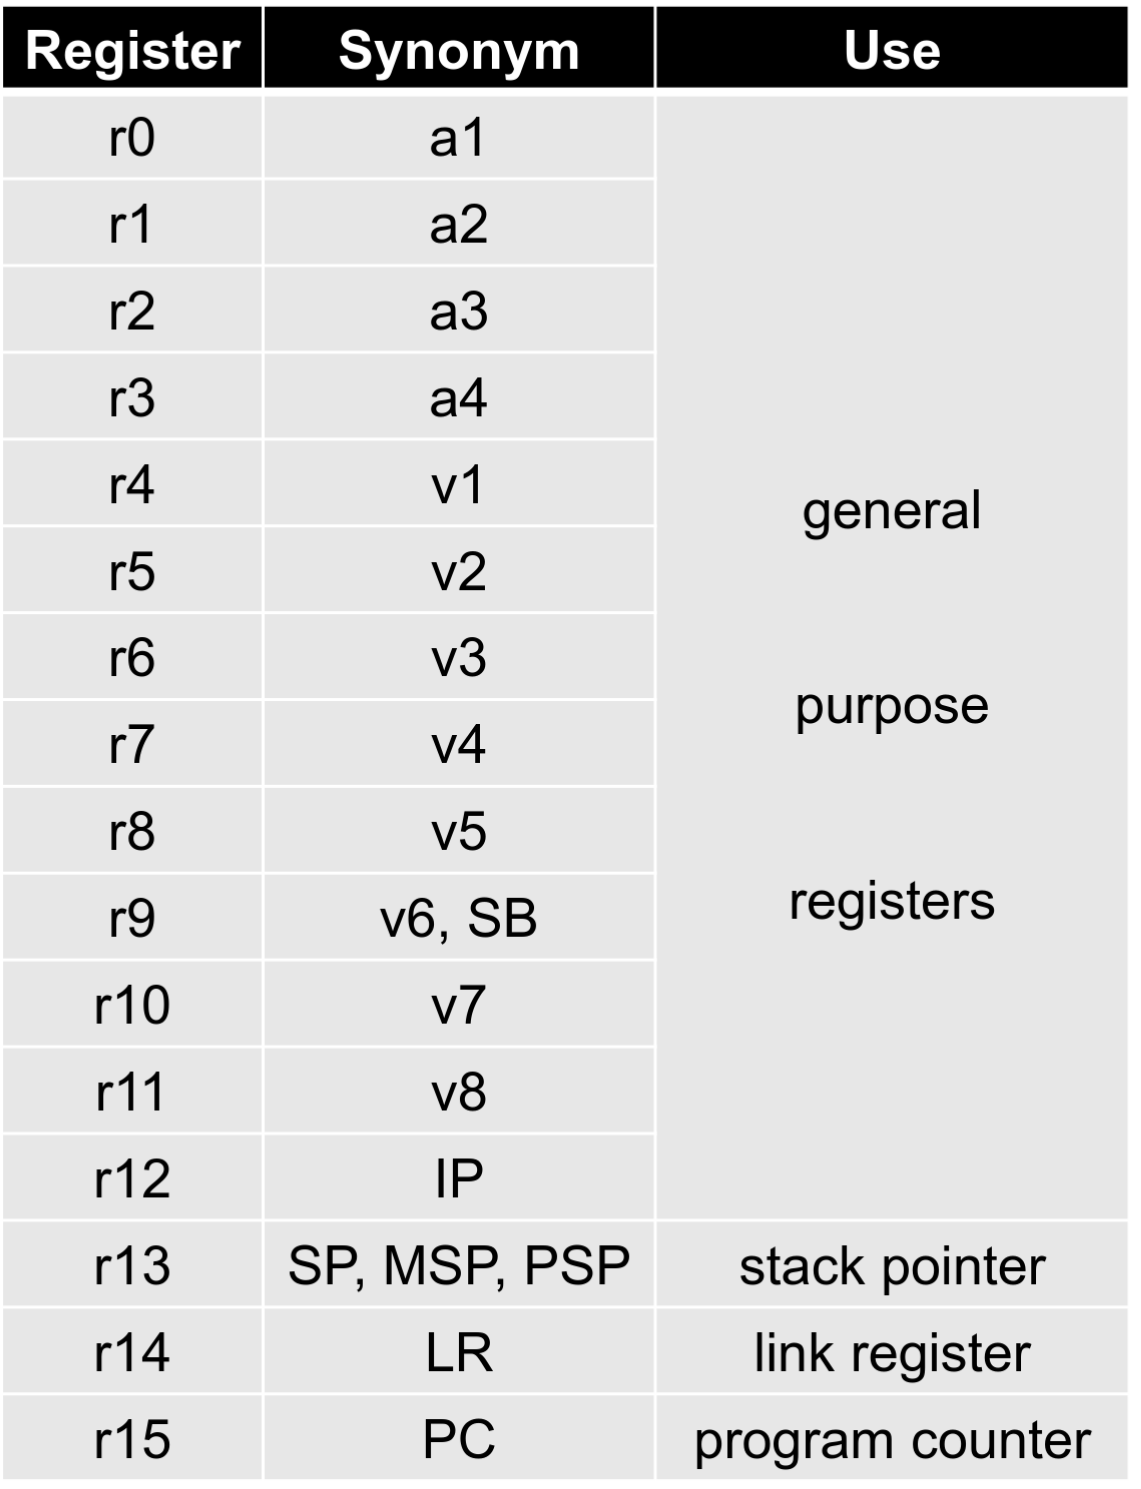
\includegraphics[scale=0.2]{../figures/arm7_gp_regs.png}
\end{center}

We sse the aliases in the table.
The main ones are:
\begin{itemize}
	\item \textbf{IP}: not really significant, means \textit{Intra-Procedure scratch} for compiler generated routines (see AAPCS below);
	\item \textbf{SP}: this is the \textit{Stack Pointer}, with \textbf{MSP} and \textbf{PSP} being respectively the \textit{Main} (handler) and \textit{Program} (thread/user) stack pointers in the respective modes;
	\item \textbf{LR}: this is the \textit{Link Register} for jump and link calling convention;
	\item \textbf{PC}: the good old program counter.
\end{itemize}

Arm defines \textbf{AAPCS} (\textit{ARM Architecture Procedure Call Standard}) for the caller convention ABI.
A quick overview is:
\begin{itemize}
	\item Registers from \texttt{r0} to \texttt{r3} are the first 4 function arguments (from the fifth onwards we use the stack). Register \texttt{r0} then takes the return value. These are \textit{caller-saved};
	\item Registers from \textit{r4} to \textit{r11} are \textit{callee-saved} scratch;
	\item Register \texttt{r12} is, as we said, a special \textit{intra-procedure scratch}. The only significant characteristic for now is that it's \textit{caller-saved}, as the first four.
\end{itemize}

\par\smallskip\textbf{\textsf{Special registers}}
We also have the following special registers:
\begin{center}
	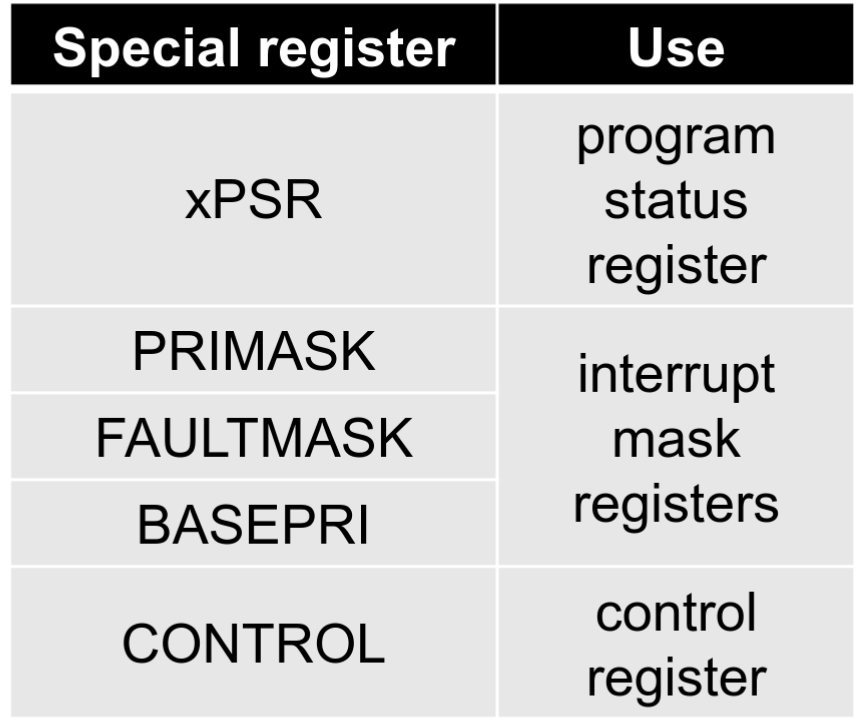
\includegraphics[scale=0.2]{../figures/arm7_sp_regs.png}
\end{center}

The \textbf{PSR} (\textit{Program Status Register}) is significant.

\begin{center}
	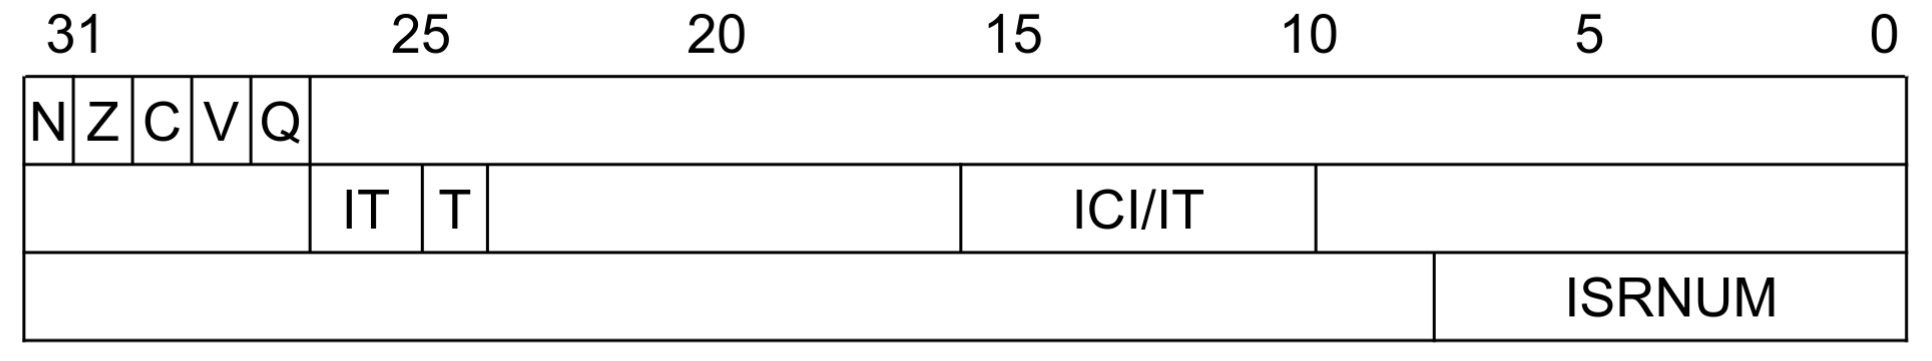
\includegraphics[scale=0.2]{../figures/xpsr.png}
\end{center}

It can be accessed all at once (PSR) or as a combination of 3 registers (in order, the three rows of the figure above):
\begin{itemize}
	\item \textit{Application Program Status Register} (\textbf{APSR}):
This contains application info (akin to the status flags on x86):
\begin{itemize}
\item N: Negative result from ALU;
\item Z: Zero result from ALU;
\item C: ALU operation Carried out;
\item V: ALU operation oVerflowed;
\item Q: “sticky” flag for saturation arithmetic.
\end{itemize}

	\item \textit{Execution Program Status Register}   (\textbf{EPSR}).
		This contains program execution status usually not of interest to the programmer:
\begin{itemize}
	\item IT: IF-THEN instruction status bits. This is interesting: the ARMv7-M (Cortex-M3) uses conditional execution to let instructions execute only when a condition is true. The IT instruction controls this for Thumb instructions;
\item ICI: Interrupt-Continuable Instruction bits;
\item T: Thumb bit. It is always 1: clearing this bit will cause a hard fault exception in ARM-v7.
\end{itemize}

\item \textit{Interrupt Program Status Register}   (\textbf{IPSR}). It contains an exception number used in exception handling. The ISRNUM is extremely important as, if it is different than 0, signals that the processor is in \textit{handler} mode (the equivalent of system mode in ARM).
\end{itemize}



\par\smallskip\textbf{\textsf{Instructions}}
There are 3 kinds of instructions:
\begin{itemize}
	\item ARM instructions: 32 bits wide
	\item Thumb instructions: 16 bits wide
	\item Thumb-2 instructions: 16 or 32 bits wide
\end{itemize}

In fact, ARM v7-M architecture supports Thumb and Thumb-2 instructions only.

\par\smallskip\textbf{\textsf{Processor modes}} 
We have orthogonal operating and privilege modes.

There are two operating modes:
\begin{itemize}
	\item Thread mode: on reset or after completing the exception routine;
	\item Handler mode: when an exception occurs.
\end{itemize}

And two access levels:
\begin{itemize}
	\item User level: limited access to resources;
	\item Privileged level: access to all resources.
\end{itemize}

Note that handler mode is always privileged.

The CONTROL register has only 2 bits, which control:
\begin{itemize}
	\item Bit 0, which is \textbf{nPRIV}, controls the access level;
	\item Bit 1, which is \textbf{SPSEL}, controls the current stack (main or process).
\end{itemize} 
The CONTROL register can be changed only in privileged mode.
When an exception is taken, the processor automatically switches to Handler mode. When the handler finishes and exception return occurs, the processor returns to Thread mode if no other exception handler should run.
This means handler state is encoded in IPSR $\neq 0$.

We show a summarizing table:
\begin{center}
	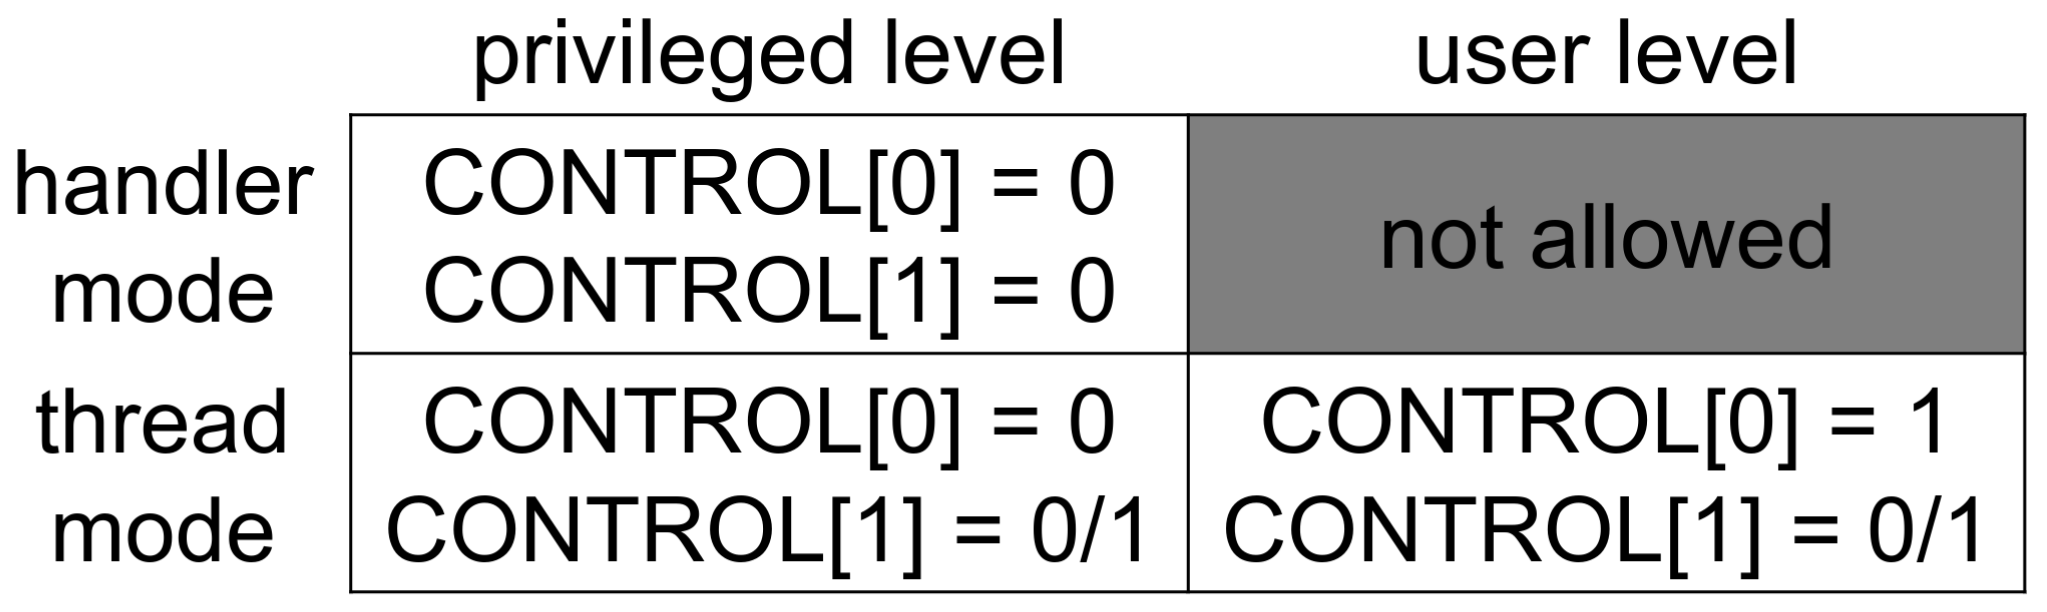
\includegraphics[scale=0.15]{../figures/control.png}
\end{center}

\par\smallskip\textbf{\textsf{Interrupt Vector Table}} ARM-v7 has an \textbf{IVT} (\textit{Interrupt Vector Table}). 
\begin{itemize}
	\item Each entry manages an exception, interrupt, or other atypical events such as a reset;
	\item The vector table contains either ARM instructions or addresses in memory: in the v7-M architecture, there are addresses.
\end{itemize}

\end{document}
